本章介绍MS-AgentNet的总体架构，并阐述所设计的包含DSConv-S和DSConv-L在内的多尺度深度可分离卷积模块；在此基础上，详细说明所提出的轻量级局部—全局融合注意力（Slim Local-Global Fusion Attention，SLFA）模块。

\subsection{MS-AgentNet总体架构与数据流}

针对现有SOH估计模型在估计精度与计算效率之间难以兼顾的问题，本文提出一种轻量级多尺度智能体网络（Multi-Scale Agent Network，MS-AgentNet）。该模型采用小核与大核深度可分离卷积提取不同时间尺度的退化特征，并结合ReLU²智能体注意力（ReLU² Agent Attention，RAA）进行跨位置全局信息交互。其中，“MS”表示由小核DSConv-S与大核DSConv-L构成的多尺度卷积设计。

MS-AgentNet的整体架构如图3-1所示。健康指标（Health Indicators，HIs）序列经滑动窗口分割后，首先通过线性嵌入层映射至$d$维特征空间；随后，嵌入特征进入MS-AgentNet Block，并在Block内依次完成局部—全局特征融合、长尺度特征细化与非线性映射。最后，模型对输出特征进行层归一化、展平和线性读出，得到SOH估计值。

\begin{figure}[H]
\centering
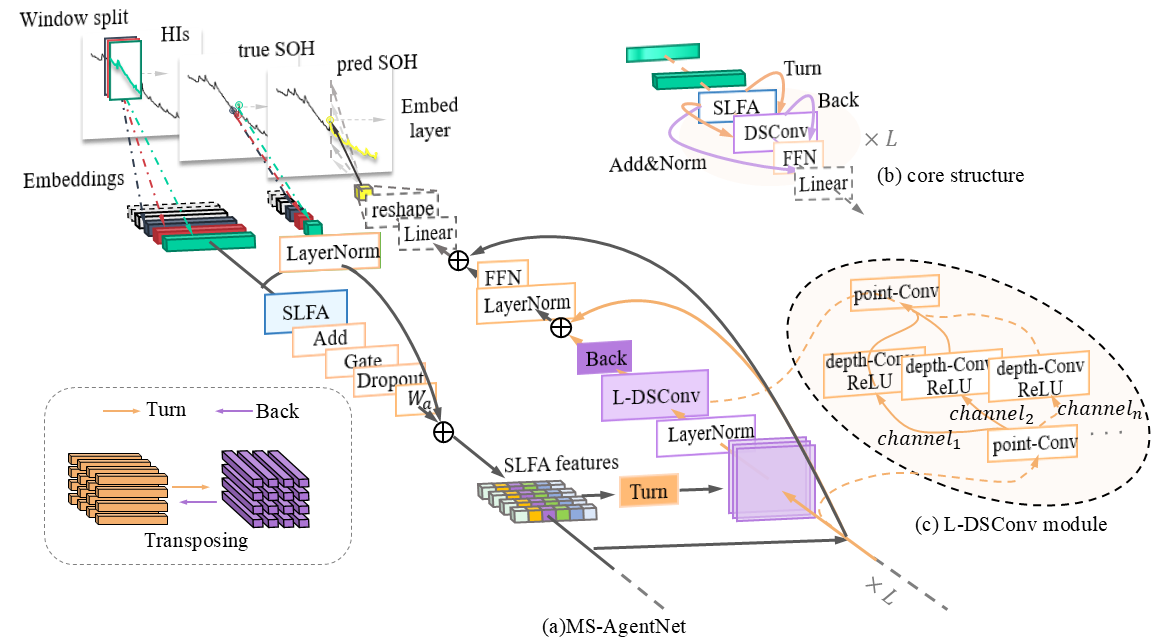
\includegraphics[width=0.92\textwidth]{figures/01.png}
\caption{Framework of MS-AgentNet. (a) Overall architecture; (b) core structure; (c) DSConv-L module.}
\label{fig:3-1}
\end{figure}


训练过程中，每个输入窗口以窗口后紧邻循环的真实SOH值作为监督标签。

从数学角度看，设第$l$个MS-AgentNet Block的输入为$\mathbf X_l\in\mathbb R^{B\times N\times d}$，其中$B$为批量大小，$N$为输入序列长度，$d$为嵌入维度。其内部特征变换可表示为以下过程：

步骤1：局部—全局融合。输入特征先由SLFA模块完成小核局部增强和智能体全局交互：

\begin{equation}
\mathbf X_l'
=
\operatorname{SLFA}(\mathbf X_l).
\tag{3-1}
\end{equation}

步骤2：长尺度特征细化。为提取较长时间尺度的退化特征，中间特征$\mathbf X_l'$先经层归一化，再通过DSConv-L模块，所得特征经可学习系数$W_l$缩放后，以残差形式与$\mathbf X_l'$相加：

\begin{equation}
\mathbf X_l''
=
\mathbf X_l'
+
W_l
\operatorname{DSConv\text{-}L}
\left(
\operatorname{LN}(\mathbf X_l')
\right).
\tag{3-2}
\end{equation}

步骤3：非线性映射。细化后的特征$\mathbf X_l''$经层归一化后输入FFN，并通过残差连接得到输出$\mathbf Y_l$：

\begin{equation}
\mathbf Y_l
=
\mathbf X_l''+
\operatorname{FFN}
\left(
\operatorname{LN}_0(\mathbf X_l'')
\right).
\tag{3-3}
\end{equation}

并令该Block的输出为$\mathbf X_{l+1}=\mathbf Y_l$。其中，$\operatorname{SLFA}(\cdot)$、$\operatorname{DSConv\text{-}L}(\cdot)$和$\operatorname{FFN}(\cdot)$分别表示轻量级局部—全局融合注意力模块、大核深度可分离卷积模块和前馈神经网络；$W_l$为可学习缩放系数，$\operatorname{LN}(\cdot)$表示层归一化，$\operatorname{LN}_0(\cdot)$表示不含可学习仿射参数的层归一化。

\subsection{所设计的多尺度深度可分离卷积模块}

本节首先介绍DSConv的基本结构，并将其与标准卷积进行计算量比较；随后说明DSConv-S和DSConv-L的结构配置及其多尺度特性。

\begin{figure}[!htb]
\centering
\noindent\makebox[\linewidth][c]{%
  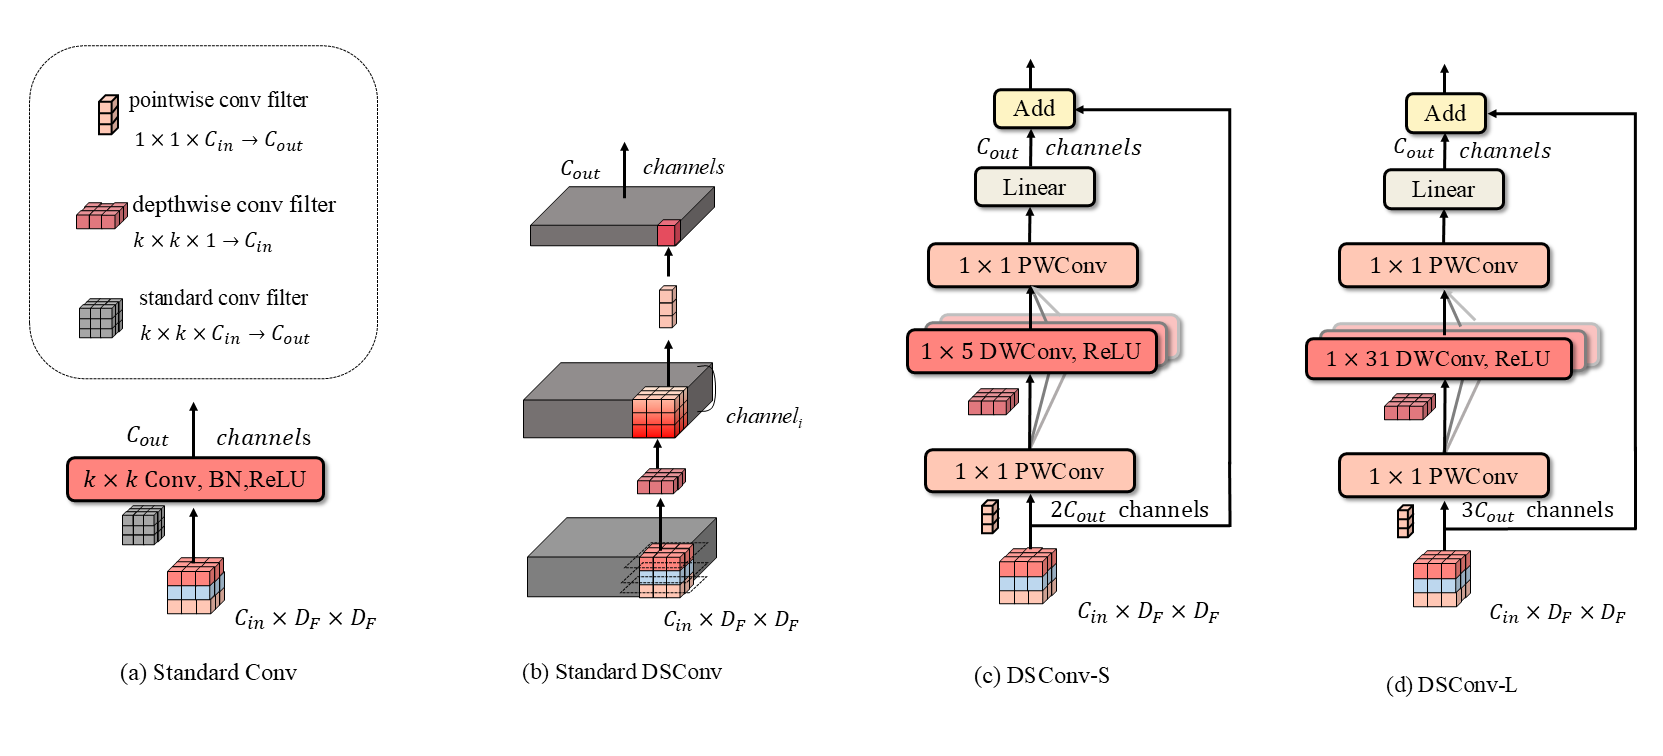
\includegraphics[width=175mm]{figures/02.png}%
}
\caption{The fundamental structures of convolutional modules: (a) standard convolution; (b) standard depthwise separable convolution; (c) DSConv-S module; and (d) DSConv-L module.}
\label{fig:3-2}
\end{figure}


\subsubsection{DSConv基本结构与计算量比较}

卷积运算通过滑动卷积核提取时间序列中的局部信息\cite{ref71}。标准卷积在所有输入通道上进行运算，每个卷积核生成一个输出特征图，对应一个输出通道。随着输入通道数、输出通道数和卷积核尺寸增加，其参数量与计算开销迅速累积，显著推高计算负载并延长训练时间。在小样本电池数据集上，较大的参数量还可能增加模型的过拟合风险。其计算成本可表示为：

\begin{equation}
C_{\mathrm{Conv}}
=
k\times k\times C_{\mathrm{in}}\times C_{\mathrm{out}}\times D_F\times D_F.
\tag{3-4}
\end{equation}

其中，$k$、$C_{\mathrm{in}}$、$C_{\mathrm{out}}$和$D_F$分别表示卷积核大小、输入通道数、输出通道数和特征图尺寸。

与标准卷积不同，深度可分离卷积（DSConv）将卷积运算分解为深度卷积和逐点卷积两个阶段\cite{ref71}。其中，深度卷积为每个输入通道单独配置卷积核，在通道内完成局部特征提取；随后，$1\times1$逐点卷积融合不同通道的特征，并将通道数调整为$C_{\mathrm{out}}$。通过分离通道内特征提取与通道间特征融合，DSConv减少了标准卷积中的密集跨通道运算。其计算成本可表示为：

\begin{equation}
C_{\mathrm{DSConv}}
=
k\times k\times C_{\mathrm{in}}\times D_F\times D_F
+
C_{\mathrm{in}}\times C_{\mathrm{out}}\times D_F\times D_F.
\tag{3-5}
\end{equation}

进一步比较两类卷积的计算量，可得二者之比为：

\begin{equation}
\begin{aligned}
\frac{C_{\mathrm{DSConv}}}{C_{\mathrm{Conv}}}
&=
\frac{
k\times k\times C_{\mathrm{in}}\times D_F\times D_F
+
C_{\mathrm{in}}\times C_{\mathrm{out}}\times D_F\times D_F
}{
k\times k\times C_{\mathrm{in}}\times C_{\mathrm{out}}\times D_F\times D_F
} \\
&=
\frac{1}{C_{\mathrm{out}}}
+
\frac{1}{k^2}.
\end{aligned}
\tag{3-6}
\end{equation}

由式（3-6）可知，在输入、输出通道配置一致的情况下，DSConv的计算成本低于标准卷积，为后续小核与大核卷积模块的构建提供了基础。

\subsubsection{DSConv-S：双重作用的局部增强}

小核DSConv-S采用紧凑的$1\times5$深度卷积，并嵌入SLFA模块、位于RAA全局交互之前，以实现输入增强与局部分支保留两项作用：

1. \textbf{输入增强。} DSConv-S提取输入特征中的局部邻域信息，形成局部增强表示$\mathbf X_S$。RAA随后基于$\mathbf X_S$构造查询、键和值，并通过智能体聚合与广播完成跨位置交互。这一前置卷积为RAA引入局部性偏置，增强其在跨位置上下文聚合过程中对局部变化的表征。

2. \textbf{局部分支保留。} 在SLFA中，$\mathbf X_S$同时传递至RAA分支和局部分支。局部分支对$\mathbf X_S$进行层归一化后传递至融合端，并与RAA分支建立的跨位置上下文进行融合，形成局部特征与全局信息的互补表示。

DSConv-S采用两倍通道扩展。输入首先经转置使特征维度对应卷积通道维度，再通过第一层$1\times1$逐点卷积完成通道扩展。随后，$1\times5$深度卷积在各通道内提取短邻域特征，并经ReLU激活；第二层$1\times1$逐点卷积进一步融合通道信息并恢复输出维度。最后，输出经逆转置后与输入通过残差连接融合。上述过程表示为：

\begin{equation}
\mathbf X_S
=
\mathbf X
+
\mathcal T^{-1}
[ 
\operatorname{PW}_{\downarrow}
(
\operatorname{ReLU}
(
\operatorname{DW}_{5}
(
\operatorname{PW}_{\uparrow}
(
\mathcal T(\mathbf X)
)
)
)
)
)].
\tag{3-7}
\end{equation}

其中，$\operatorname{PW}_{\uparrow}$和$\operatorname{PW}_{\downarrow}$分别表示通道扩展和通道恢复的逐点卷积，$\operatorname{DW}_{5}$表示尺寸为$1\times5$的深度卷积，$\mathcal T(\cdot)$与$\mathcal T^{-1}(\cdot)$分别表示转置和逆转置操作。为便于后文表述，将上述过程简记为

\begin{equation*}
\mathbf X_S=\operatorname{DSConv\text{-}S}(\mathbf X).
\end{equation*}

\textbf{计算分析。} 在两倍通道扩展条件下，DSConv-S的计算成本主要来自两层$1\times1$逐点卷积和一层$1\times5$深度卷积，可表示为：

\begin{equation*}
C_{\mathrm{in}}\times2C_{\mathrm{out}}\times D_F\times D_F
+1\times5\times2C_{\mathrm{out}}\times D_F\times D_F
+2C_{\mathrm{out}}\times C_{\mathrm{out}}\times D_F\times D_F,
\end{equation*}

其中，$2C_{\mathrm{out}}$和$D_F\times D_F$分别表示扩展后的通道数和特征图尺寸。

\subsubsection{DSConv-L：后融合长尺度细化}

大核DSConv-L作为独立的特征细化模块置于SLFA之后。凭借较大的感受野，DSConv-L提取融合表示中较长时间尺度的退化特征，并完成后融合细化。

DSConv-L同样按照“通道扩展—卷积特征提取—通道恢复”的顺序组织，并采用三倍通道扩展和$1\times31$深度卷积。其计算过程表示为：

\begin{equation}
\operatorname{DSConv\text{-}L}(\mathbf X)
=
\mathcal T^{-1}
[ 
\operatorname{PW}_{L,\mathrm{out}}
(
\operatorname{ReLU}
(
\operatorname{DW}_{31}
(
\operatorname{PW}_{L,\uparrow}
(
\mathcal T(\mathbf X)
)
)
)
)
)].
\tag{3-8}
\end{equation}

其中，$\operatorname{PW}_{L,\uparrow}$和$\operatorname{PW}_{L,\mathrm{out}}$分别表示通道扩展和通道恢复的逐点卷积，$\operatorname{DW}_{31}$表示尺寸为$1\times31$的大核深度卷积。

\textbf{计算分析。} 在三倍通道扩展条件下，DSConv-L的计算成本可表示为：

\begin{equation*}
C_{\mathrm{in}}\times3C_{\mathrm{out}}\times D_F\times D_F
+1\times31\times3C_{\mathrm{out}}\times D_F\times D_F
+3C_{\mathrm{out}}\times C_{\mathrm{out}}\times D_F\times D_F,
\end{equation*}

其中，$3C_{\mathrm{out}}$和$D_F\times D_F$分别表示扩展后的通道数和特征图尺寸。

\subsection{所提出的轻量级局部—全局融合注意力模块}

本节给出多头自注意力的一般形式，简要比较Softmax注意力与线性注意力，并在此基础上介绍所提出的SLFA模块。该模块兼顾局部—全局特征建模与计算效率。

\begin{figure}[htbp]
\centering
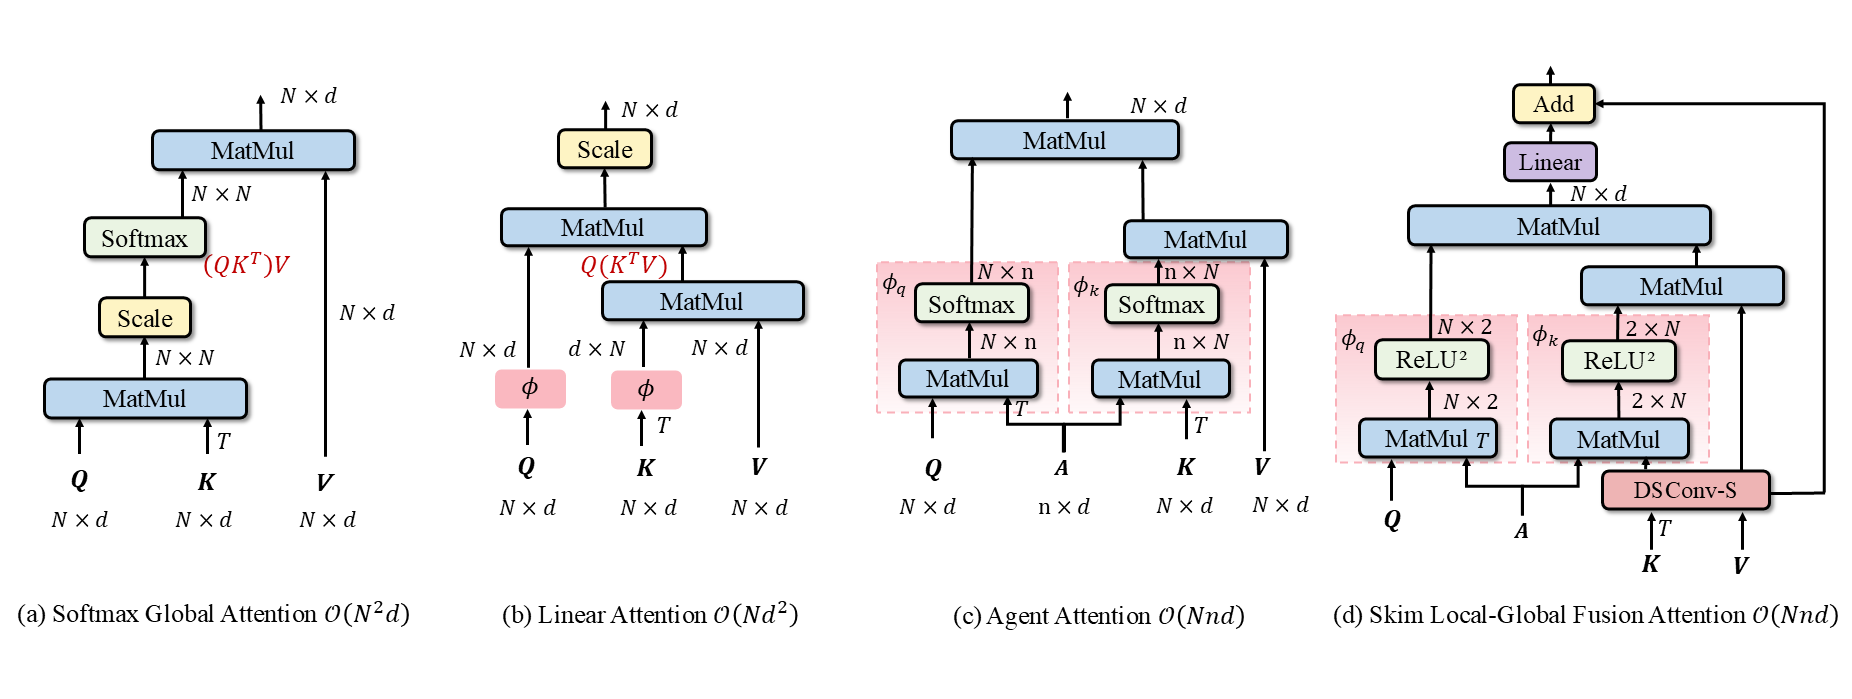
\includegraphics[width=0.92\textwidth]{figures/fig3_3_attention_comparison.png}
\caption{不同注意力机制的结构对比：（a）Softmax注意力；（b）线性注意力；（c）智能体注意力；（d）所提出的SLFA模块。}
\label{fig:3-3}
\end{figure}


\subsubsection{多头自注意力的一般形式}

多头自注意力通过多个并行注意力头在不同表示子空间内计算特征之间的相关性\cite{ref34}。设输入特征为$\mathbf X\in\mathbb R^{N\times d}$，第$i$个注意力头的查询、键和值表示为：

\begin{equation}
\mathbf Q_i=\mathbf X\mathbf W_i^Q,\qquad
\mathbf K_i=\mathbf X\mathbf W_i^K,\qquad
\mathbf V_i=\mathbf X\mathbf W_i^V.
\tag{3-9}
\end{equation}

其中，$N$为序列长度，$d$为输入特征维度，$\mathbf W_i^Q,\mathbf W_i^K,\mathbf W_i^V\in\mathbb R^{d\times d_h}$为可学习投影矩阵，$i=1,2,\ldots,h$，$h$为注意力头数，$d_h=d/h$为单个注意力头的特征维度。

在采用非负相似度函数构造归一化注意力权重时，第$i$个注意力头在第$p$个位置的输出可表示为：

\begin{equation}
\mathbf O_{i,p}
=
\frac{
\displaystyle\sum_{j=1}^{N}
\operatorname{Sim}\left(\mathbf Q_{i,p},\mathbf K_{i,j}\right)\mathbf V_{i,j}
}{
\displaystyle\sum_{j=1}^{N}
\operatorname{Sim}\left(\mathbf Q_{i,p},\mathbf K_{i,j}\right)
},
\qquad p=1,2,\ldots,N.
\tag{3-10}
\end{equation}

其中，$\mathbf Q_{i,p}$表示第$i$个注意力头中第$p$个位置的查询，$\mathbf K_{i,j}$和$\mathbf V_{i,j}$分别表示第$j$个位置的键和值，$\operatorname{Sim}(\cdot,\cdot)$表示非负相似度函数\cite{ref40}。

所有位置的输出共同构成第$i$个注意力头的输出矩阵$\mathbf O_i\in\mathbb R^{N\times d_h}$，各注意力头的输出随后沿特征维度拼接。不同注意力机制的主要区别在于相似度函数及其计算顺序。

\subsubsection{Softmax注意力与线性注意力}

标准Softmax注意力通过查询与键的点积计算序列位置之间的相关性，并利用Softmax函数对相关性得分进行归一化\cite{ref34}。第$i$个注意力头的输出可表示为：

\begin{equation}
\mathbf O_i
=
\operatorname{Softmax}
\left(
\frac{\mathbf Q_i\mathbf K_i^{\mathrm T}}{\sqrt{d_h}}
\right)
\mathbf V_i.
\tag{3-11}
\end{equation}

Softmax中的指数映射与归一化使相关性较高的查询—键对获得更大的注意力权重\cite{ref34}。然而，$\mathbf Q_i\mathbf K_i^{\mathrm T}$需要计算所有查询与键之间的两两关系，并形成尺寸为$N\times N$的注意力矩阵。因此，单个注意力头的计算复杂度为$O(N^2d_h)$，相关性矩阵的存储复杂度为$O(N^2)$；随着序列长度增加，其计算与存储开销会显著增大\cite{ref34,ref39}。

针对Softmax注意力的二次计算开销，线性注意力利用核函数$\phi(\cdot)$映射查询和键，并借助矩阵乘法结合律重新组织计算顺序\cite{ref40}。第$i$个注意力头的输出可写为：

\begin{equation}
\mathbf O_i
=
\frac{
\phi(\mathbf Q_i)
\left[
\phi(\mathbf K_i)^{\mathrm T}\mathbf V_i
\right]
}{
\phi(\mathbf Q_i)
\left[
\phi(\mathbf K_i)^{\mathrm T}\mathbf 1
\right]
}.
\tag{3-12}
\end{equation}

其中，$\phi(\cdot)$表示非负特征映射，例如$\phi(\mathbf x)=\operatorname{ELU}(\mathbf x)+1$；$\mathbf 1$表示全1向量，用于计算对应的归一化项\cite{ref40}。

通过优先计算$\phi(\mathbf K_i)^{\mathrm T}\mathbf V_i$，线性注意力避免了完整$N\times N$注意力矩阵的构造。当特征映射维度与$d_h$一致时，其计算复杂度为$O(Nd_h^2)$；当$d_h$固定时，该复杂度关于序列长度$N$为线性\cite{ref40}。

线性注意力以较低计算复杂度完成全局信息交互，但其计算过程未显式引入局部邻域特征\cite{ref31,ref39,ref40,ref64}。因此，需要进一步协同建模跨位置交互与局部特征。

\subsubsection{所提出的SLFA模块}

为同时捕获局部邻域特征与跨位置交互，本文将DSConv-S与所构建的ReLU²智能体注意力（ReLU² Agent Attention，RAA）相结合，提出SLFA模块，其结构如图3-3（d）所示。该模块采用局部分支与RAA分支的融合形式：DSConv-S首先提取局部表示，RAA随后以该表示为输入完成跨位置特征交互，两个分支的输出经加法融合。

\textbf{（1）ReLU²智能体注意力。}

Agent Attention以少量智能体作为信息中介，将序列位置之间的全局交互分解为上下文聚合与信息广播两个阶段\cite{ref46}：智能体首先从键和值中聚合序列上下文，各查询位置随后从智能体上下文中读取信息。标准Agent Attention在两个阶段均采用Softmax归一化，本文则采用ReLU²行归一化，以抑制非正相关性并突出高相关性位置，由此构建RAA。

为降低查询、键和值生成过程中的参数开销，RAA采用可学习通道缩放调节不同特征通道的相对贡献，并将缩放后的特征划分至各注意力头：

\begin{equation}
\mathbf Q_i=\operatorname{Split}_i(\mathbf X\odot\mathbf s_q),\quad
\mathbf K_i=\operatorname{Split}_i(\mathbf X\odot\mathbf s_k),\quad
\mathbf V_i=\operatorname{Split}_i(\mathbf X\odot\mathbf s_v).
\tag{3-13}
\end{equation}

其中，$\mathbf s_q,\mathbf s_k,\mathbf s_v\in\mathbb R^d$为可学习通道缩放向量，$\odot$表示逐元素相乘，$\operatorname{Split}_i(\cdot)$表示沿特征维度划分为$h$个$d_h$维子空间并取第$i$个子空间。

相较于标准查询、键和值线性投影约$3d^2$的参数量，三组通道缩放向量仅包含$3d$个参数，从而降低了查询、键和值生成过程中的参数开销。

RAA设置$n_a=2$个可学习智能体，并以全局共享的静态矩阵$\mathbf A\in\mathbb R^{n_a\times d}$表示。

沿特征维度将全局智能体矩阵$\mathbf A$划分为$h$个子空间，第$i$个注意力头对应的智能体表示为$\mathbf A_i=\operatorname{Split}_i(\mathbf A)\in\mathbb R^{n_a\times d_h}$。聚合与广播阶段均采用ReLU²行归一化：

\begin{equation}
\left[\mathcal R_2(\mathbf Z)\right]_{r,c}
=
\begin{cases}
\dfrac{\operatorname{ReLU}(\mathbf Z_{r,c})^2}
{\sum_{j=1}^{M}\operatorname{ReLU}(\mathbf Z_{r,j})^2},
&
\sum_{j=1}^{M}\operatorname{ReLU}(\mathbf Z_{r,j})^2>0,\\[10pt]
\dfrac{1}{M},
&
\sum_{j=1}^{M}\operatorname{ReLU}(\mathbf Z_{r,j})^2=0.
\end{cases}
\tag{3-14}
\end{equation}

其中，$M$表示每一行参与归一化的元素数量：在智能体聚合阶段，$M=N$；在信息广播阶段，$M=n_a$。ReLU截断非正相关性得分，平方操作进一步扩大正相关性得分之间的差异，使归一化权重更加突出高相关性位置。当某一行不存在正相关性得分时，$\mathcal R_2(\cdot)$返回均匀分布，以保持归一化结果的有效性。

在智能体聚合阶段，$\mathbf A_i$作为查询，从序列的键和值中汇集上下文：

\begin{equation}
\boldsymbol{\Phi}_{k,i}
=
\mathcal R_2
\left(
\frac{\mathbf A_i\mathbf K_i^{\mathrm T}}{\sqrt{d_h}}
\right),
\qquad
\mathbf V_{A,i}
=
\boldsymbol{\Phi}_{k,i}\mathbf V_i.
\tag{3-15}
\end{equation}

其中，$\boldsymbol{\Phi}_{k,i}\in\mathbb R^{n_a\times N}$表示智能体对各序列位置的聚合权重，$\mathbf V_{A,i}\in\mathbb R^{n_a\times d_h}$表示聚合得到的智能体上下文。

在信息广播阶段，各查询位置根据自身特征从智能体上下文中读取信息：

\begin{equation}
\boldsymbol{\Phi}_{q,i}
=
\mathcal R_2
\left(
\frac{\mathbf Q_i\mathbf A_i^{\mathrm T}}{\sqrt{d_h}}
\right),
\qquad
\mathbf O_i
=
\boldsymbol{\Phi}_{q,i}\mathbf V_{A,i}.
\tag{3-16}
\end{equation}

其中，$\boldsymbol{\Phi}_{q,i}\in\mathbb R^{N\times n_a}$表示各查询位置对智能体的广播权重，$\mathbf O_i\in\mathbb R^{N\times d_h}$为第$i$个注意力头的输出。由于广播权重沿智能体维度逐行归一化，不同查询位置能够形成各自的智能体权重分配。

由式（3-15）和式（3-16）可知，从等效映射角度看，第$i$个注意力头中智能体介导的序列交互可表示为$\boldsymbol{\Phi}_{q,i}\boldsymbol{\Phi}_{k,i}\in\mathbb R^{N\times N}$，其秩不超过智能体数量$n_a$。

各注意力头的输出沿特征维度拼接，并通过可学习输出缩放向量$\mathbf s_o$调节通道响应，随后与输入特征进行残差相加：

\begin{equation}
\operatorname{RAA}(\mathbf X)
=
\mathbf X+
\operatorname{Concat}(\mathbf O_1,\ldots,\mathbf O_h)\odot\mathbf s_o.
\tag{3-17}
\end{equation}

其中，$\operatorname{Concat}(\cdot)$表示沿特征维度拼接各注意力头的输出，$\mathbf s_o\in\mathbb R^d$为可学习输出缩放向量。式（3-17）通过残差连接融合输入特征与多头智能体交互结果。

RAA在聚合与广播阶段分别生成$n_a\times N$和$N\times n_a$相关性矩阵。由此，单个注意力头的计算复杂度为$O(Nn_ad_h)$，$h$个注意力头的总计算复杂度为$O(Nn_ad)$，相关性权重的存储规模为$O(hNn_a)$。当$h$和$n_a$固定时，计算量与存储量均随序列长度$N$线性增长。

\textbf{（2）局部—全局特征融合。}

输入特征$\mathbf X$首先经DSConv-S得到局部表示$\mathbf X_S=\operatorname{DSConv\text{-}S}(\mathbf X)$，随后分别进入局部分支和RAA分支。局部分支对$\mathbf X_S$进行层归一化，RAA分支通过智能体聚合与信息广播建立跨位置特征交互。SLFA的融合输出$\mathbf X_F$计算如下：

\begin{equation}
\mathbf X_F
=
\operatorname{LN}(\mathbf X_S)
+
W_a
\operatorname{Dropout}
\left(
\operatorname{RAA}(\mathbf X_S)
\right).
\tag{3-18}
\end{equation}

其中，$\mathbf X_F$表示SLFA的融合输出，$\operatorname{LN}(\mathbf X_S)$为局部分支的归一化表示，$\operatorname{RAA}(\mathbf X_S)$为RAA分支输出；$\operatorname{Dropout}(\cdot)$用于训练阶段的正则化\cite{ref75}，$W_a$为调节RAA分支贡献的可学习缩放系数。

这种加性连接保留了DSConv-S提取的局部退化特征，并融合RAA建立的跨位置上下文，在形成局部—全局联合表示的同时，保持关于序列长度$N$的线性计算复杂度。
